\chapter{混沌信号的稀疏重构算法}
在实际情况下,混沌信号总会被噪声污染,又由于混沌信号的非周期、宽带频谱等特性,使得一些现有的信号重构方法在处理混沌信号时难以获得理想的效果。
为此,本章基于稀疏重构理论提出了一种针对被噪声污染混沌信号的重构算法,而随后的以第3章提出的Duffing-WS小世界网络输出混沌信号为例的仿真实验也表明,该方法能较为稳健地恢复受噪声干扰的Duffing-WS型小世界网络输出的带噪混沌信号,不仅较具有更高的输出信噪比, 而原始信号的混沌特性也能得到较大程度的恢复,这是一般稀疏重构算法不具有的。

\section{基于稀疏重构的混沌信号重构算法}
设Duffing-WS小世界网络某个节点输出的离散化带噪混沌信号序列为:
\begin{equation}
    u[n]=x[n]+w[n], n=1,2, \ldots, N
\end{equation}
其中 $x[n]$ 为原始混沌序列, $w[n]$ 为零均值和方差为 $\sigma$ 的高斯白噪声。因此,方程又写成矢量形式为:
\begin{equation}
    \boldsymbol{u}=\boldsymbol{x}+\boldsymbol{w}
\end{equation}

我们知道 Duffing-WS 小世界网络输出的混沌信号在时域上并不是稀疏信号,
但它可能具有某类特定的变换基 $\Psi$, 使得在此基上的变换系数服从幂指数递减,
这也说明该信号在此变换域中具有较强的可压缩性。
这里不妨假设 $\boldsymbol{x}=\Psi \boldsymbol{a}, \boldsymbol{a}$ 为稀疏表示系数,
我们保留所有系数中绝对值最大的 $s$ 个系数得到 真正的稀疏系数 $\hat{\boldsymbol{a}}_s$,
基于稀疏重构理论的混沌信号重构问题便是需要求解如下 的 基于$l_1$ 范数的稀疏重构最优化问题:
\begin{equation}
    \min \left\|\hat{\boldsymbol{a}}_s\right\|_1, \text { s.t., }\left\|\Psi \hat{\boldsymbol{a}}_s-\boldsymbol{y}\right\|_2 \leq \boldsymbol{\varepsilon}
\end{equation}\par
我们知道,基于$l_1$范数的稀疏重构算法有利于保持信号的稀疏性,也称为基追踪算法。目前针对该问题的重构算法主要可归为凸优化算法、贪婪算法和
组合算法三大类。其中,贪婪算法通过每次迭代时选择一个局部最优解来逐步逼近原始信号,简单、易于理解且快速方便。
典型的贪婪算法有匹配追踪(MP)算法,而改进的有正交匹配追踪(OMP)算法和压缩采样匹配追踪(CoSaMP)算法等。
压缩采样匹配追踪(CoSaMP)算法是由Needell与Tropp提出的一个针对OMP的改进算法,具有比MP和OMP更好的数值表现,
该算法是结合OMP思想与采样技巧,在每次迭代中将一些随机样本加入到选定的支撑集中,并采用最小二乘法对所选支撑集进行解的估计。

本章考虑基于 CoSaMP 算法对带噪的混沌信号进行重构, 其中而稀疏变换基 选择离散傅里叶变换基。
这是因为混沌信号虽然具有时域类随机性但它认可看成低频信号,因此其傅里叶系数在高频区域将大幅度衰减,
因此我们可将其高频傅里叶系数置零将其离散信号转换为近似稀疏向量。算法如下\par
(1)初始化输出信号 $\boldsymbol{a}^0 \leftarrow \mathbf{0}$, 将当前的采样信号作为初始值 $\boldsymbol{v} \leftarrow \boldsymbol{u}$\par
(2)迭代变量 $k \leftarrow 0$\par
(3)进入循环: $k \leftarrow k+1$\par
计算内积 $\boldsymbol{y} \leftarrow \boldsymbol{\Phi}^* \boldsymbol{v}$\par
\par 确定支撑集 (2 倍稀疏度 $) \boldsymbol{\Omega} \leftarrow \operatorname{supp}\left(\mathbf{y}_{2 \mathrm{~s}}\right), \boldsymbol{T} \leftarrow \boldsymbol{\Omega} \cup \operatorname{supp}\left(\boldsymbol{a}^{k-1}\right)$
\par 运用最小二乘法给出取值 $\left.\boldsymbol{b}\right|_T \leftarrow \boldsymbol{\Phi}_T \boldsymbol{u},\left.\boldsymbol{b}\right|_{T^c} \leftarrow \mathbf{0}$
\par 更新输出信号 $\boldsymbol{a}^k \leftarrow \boldsymbol{b}_s$
\par 更新残差 $\boldsymbol{v} \leftarrow \boldsymbol{u}-\boldsymbol{\Phi} \boldsymbol{a}^k$
\par 直至 $k=s$ 跳出, 输出 $\boldsymbol{a}$ 。

算法的输入为采样矩阵 $\boldsymbol{\Phi}$ (这里设置为高斯随机矩阵)和 采样信号 $\boldsymbol{u}$
(即 Duffing-WS小世界网络某个节点输出的带噪混沌信号), 并假设采样信号截断处理后的傅里叶基表示系数 $\boldsymbol{a}$
的稀疏度为 $s$; 算法的输出为 $s$ 维的 压缩后的信号 $\boldsymbol{a}$, 利用傅里叶逆变换即可重构原始混沌信号。


\section{仿真分析}
这一节我们给出用OMP和CoSaMP两种稀疏重构算法对混沌信号的稀疏采样后还原的仿真结果对比和分析,其中混沌信号选择为模型
Duffing-WS小世界网络第一个节点的输出,并叠加一定强度的高斯白噪声。\par
\begin{figure}[!htbp]
    \centering
    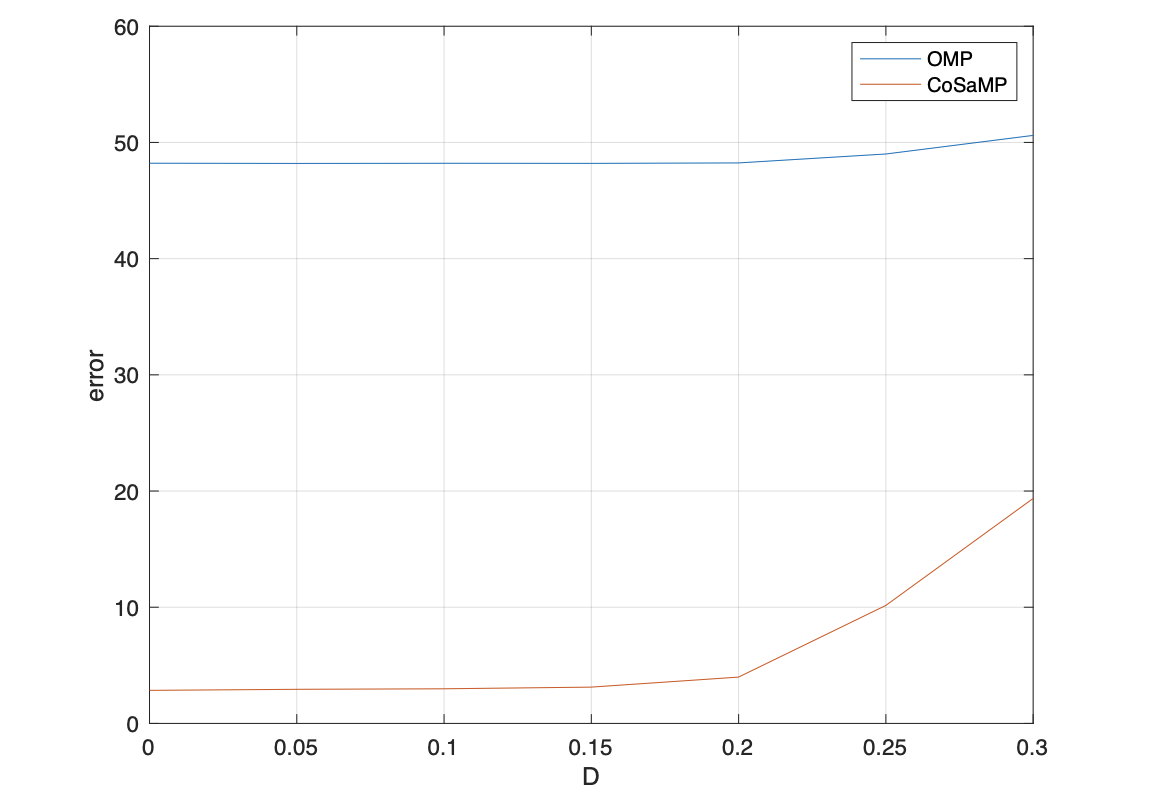
\includegraphics[width=0.7\textwidth]{42.png}
    \caption{OMP和CoSaMP两种算法的去噪能力}
\end{figure}
图(4.1)给出了OMP和CoSaMP两种算法的重构误差关于噪声强度的变化图,其中重构误差定义为重构输出信号和真实信号差的$l_2$范数。可以看到,CoSaMP算法在噪声强度小于0.2时具有非常低的重构误差,
即较好的抗噪重构性能,但之后因噪声强度的增加其误差有快速增长,但其重构性能始终优于经典的OMP算法。
经典的OMP算法对于混沌信号始终存在较大的重构误差。由此可见,CoSaMP算法相较于传统OMP算法有更出色的重构抗噪声能力。\par
\begin{figure}[!htbp]
    \centering
    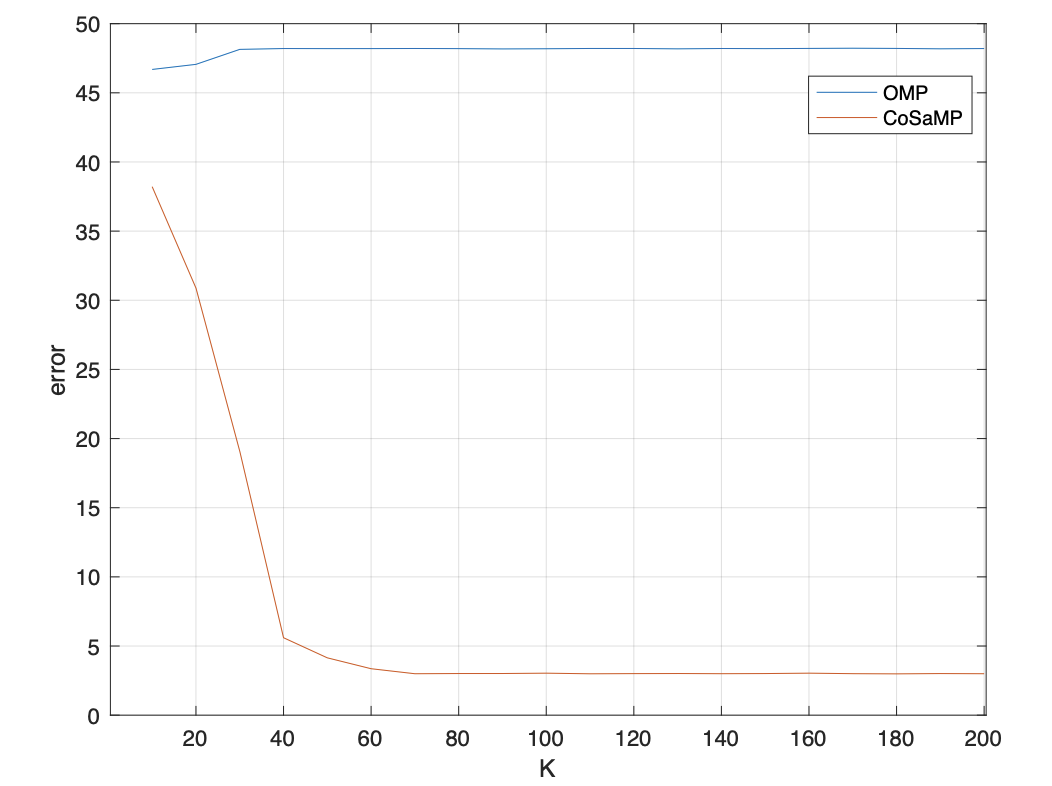
\includegraphics[width=0.7\textwidth]{43.png}
    \caption{OMP和CoSaMP两种算法的重构误差}
\end{figure}

图(4.2)则给出了选择不同稀疏度$K$值时,OMP和CoSaMP两种算法相应的重构误差。可以看出,CoSaMP算法在稀疏度增加时重构误差显著减小,
在$K = 60$左右趋于稳定,也说明该混沌信号经过离散傅里叶变换之后的稀疏系数取为$K = 60$即可较为稳健地恢复该信号,
而OMP算法对该混沌信号的重构能力一直不佳。\par
由此可见,含噪声的混沌信号稀疏重构问题目前尚未有完善的研究,常规的稀疏重构算法也对混沌信号的重构性能不佳,
以OMP算法为例,该算法在常规情况有很好的性能,但是在混沌信号情形的效果不佳。因此对混沌信号重构对传统稀疏重构算法提出了新的挑战。
\section{小结}
混沌信号作为复杂网络常见的输出形式,构建相应混沌信号在噪声干扰下的重构方法,对复杂网络的混沌控制和混沌信号的各种应用都具有重要的意义。
本章针对复杂网络输出的混沌信号,运用稀疏采样还原算法成功压缩且高精度还原了带噪声的混沌信号,并且对比了不同算法和在混沌信号情形下的性能。
仿真实验表明, 该方法能较为稳健地恢复受噪声干扰的Duffing-WS型小世界网络输出的带噪混沌信号,不仅较具有更高的输出信噪比, 而原始信号的混沌特性也能得到较大程度的恢复,
这是一般稀疏重构算法不具有的。